\documentclass[../../main/main.tex]{subfiles}
\graphicspath{{./figures/}}

\dominitoc
\faketableofcontents

\renewcommand{\mtcSfont}{\small\bfseries}
\renewcommand{\mtcSSfont}{\footnotesize}

\makeatletter
\renewcommand{\@chapapp}{Chimie -- chapitre}
\makeatother

% \toggletrue{student}
% \toggletrue{corrige}
% \renewcommand{\mycol}{black}
% \renewcommand{\mycol}{gray}

\hfuzz=5.002pt

\begin{document}
\setcounter{chapter}{5}

\settype{prof}
\settype{stud}
\settype{book}

\chapter{R\'eactions d'oxydo-r\'eduction}

\vspace*{\fill}

\begin{prgm}
	\small
	\begin{tcb}*(ror)"know"{Savoirs}
		\begin{itemize}
			\item Oxydants et réducteurs, réactions d'oxydoréduction, nombre
			      d'oxydation, dismutation et médiamutation.
			\item Exemples d'oxydants et de réducteurs minéraux usuels : nom, nature
			      et formule des ions thiosulfate, permanganate, hypochlorite, du
			      peroxyde d'hydrogène.
			\item Pile, tension à vide, potentiel d'électrode, formule de
			      \textsc{Nernst}, électrodes de référence.
			\item Diagrammes de prédominance ou d'existence.
			\item Aspect thermodynamique des réactions d'oxydo-réduction.
		\end{itemize}
	\end{tcb}
	\begin{tcb}*(ror)"how"{Savoir-faire}
		\begin{itemize}
			\item Relier la position d'un élément dans le tableau périodique et le
			      caractère oxydant ou réducteur du corps simple correspondant.

			\item Prévoir les nombres d'oxydation extrêmes d'un élément à partir de sa
			      position dans le tableau périodique.

			\item Identifier l'oxydant et le réducteur d'un couple.

			\item Décrire le fonctionnement d'une pile à partir d'une mesure de
			      tension à vide ou à partir des potentiels d'électrode.

			\item Utiliser les diagrammes de prédominance ou d'existence pour prévoir
			      les espèces incompatibles ou la nature des espèces majoritaires.

			\item Prévoir qualitativement ou quantitativement le caractère
			      thermodynamiquement favorisé ou défavorisé d'une réaction
			      d'oxydo-réduction à partir des potentiels standard des couples.
		\end{itemize}
	\end{tcb}
\end{prgm}

\vspace*{\fill}
\minitoc
\vspace*{\fill}

\newpage

\vspace*{\fill}
% {
\begin{boxes}
	\small
	\begin{tcb}(defi)<lftt>{Liste des définitions}
		\tcblistof[\paragraph*]{defi}{\hspace*{6pt}}
	\end{tcb}
	% \begin{tcb}(rapp)<lftt>{Liste des rappels}
	% 	\tcblistof[\paragraph*]{rapp}{\hspace*{6pt}}
	% \end{tcb}
	\begin{tcb}(prop)<lftt>{Liste des propriétés}
		\tcblistof[\paragraph*]{prop}{\hspace*{6pt}}
		% \tcblistof[\paragraph*]{loi}{\hspace*{6pt}}
		\tcblistof[\paragraph*]{theo}{\hspace*{6pt}}
	\end{tcb}
	% \begin{tcb}(coro)<lftt>{Liste des corollaires}
	% 	\tcblistof[\paragraph*]{coro}{\hspace*{6pt}}
	% \end{tcb}
	% \begin{tcb}(demo)<lftt>{Liste des démonstrations}
	% 	\tcblistof[\paragraph*]{demo}{\hspace*{6pt}}
	% 	\tcblistof[\paragraph*]{prev}{\hspace*{6pt}}
	% \end{tcb}
	% \begin{tcb}(inte)<lftt>{Liste des interprétations}
	% 	\tcblistof[\paragraph*]{inte}{\hspace*{6pt}}
	% \end{tcb}
	% \begin{tcb}(tool)<lftt>{Liste des outils}
	% 	\tcblistof[\paragraph*]{tool}{\hspace*{6pt}}
	% \end{tcb}
	% \begin{tcb}(nota)<lftt>{Liste des notations}
	% 	\tcblistof[\paragraph*]{nota}{\hspace*{6pt}}
	% \end{tcb}
	\begin{tcb}(appl)<lftt>{Liste des applications}
		\tcblistof[\paragraph*]{appl}{\hspace*{6pt}}
	\end{tcb}
	\begin{tcb}(rema)<lftt>{Liste des remarques}
		\tcblistof[\paragraph*]{rema}{\hspace*{6pt}}
	\end{tcb}
	\begin{tcb}(exem)<lftt>{Liste des exemples}
		\tcblistof[\paragraph*]{exem}{\hspace*{6pt}}
	\end{tcb}
	\begin{tcb}(ror)<lftt>{Liste des points importants}
		\tcblistof[\paragraph*]{ror}{\hspace*{6pt}}
	\end{tcb}
	\begin{tcb}(impo)<lftt>{Liste des erreurs communes}
		\tcblistof[\paragraph*]{impo}{\hspace*{6pt}}
	\end{tcb}
\end{boxes}
% }
\vspace*{\fill}
\newpage

\section{Oxydants et réducteurs}

\subsection{Couples oxydo-réducteurs}
\begin{tcb*}(defi){Oxydant et réducteur}
	\begin{itemize}
		\bitem{Un oxydant} est une espèce chimique capable de \xul{\psw{capter}} un
		ou plusieurs électrons~;
		\bitem{Un réducteur} est une espèce chimique capable de \xul{\psw{céder}} un
		ou plusieurs électrons~;
		\bitem{Un couple} oxydant-réducteur, noté Ox/Red\ftn{On fera donc
			particulièrement au sens qui n'est pas «~redox~»~!}, est associé
		\textit{via} la \textbf{demi-équation} électronique~:
		\psw{
			\[
				\ce{Red} \ce{=} \ce{Ox} + ne^-
			\]
		}
		\vspace{-15pt}
	\end{itemize}
\end{tcb*}
\begin{tcb*}(exem)<lftt>{Couples simples}
	\begin{itemize}
		\item
		      \leftcentersright{%
		      Le cuivre~:
		      }{%
		      \psw{$\ce{Cu_{\rm(s)} = Cu^2+_{\rm(aq)} + 2e^-}$}
		      }{%
		      % \ce{Cu^2+} est un \xul{\psw{oxydant}}, \ce{Cu} est un \xul{\psw{réducteur}}
		      \ce{Cu^2+} \xul{\psw{oxydant}}, \ce{Cu} \xul{\psw{réducteur}}
		      }%
		      \vspace{-12pt}
		\item
		      \leftcentersright{%
		      Le zinc~:
		      }{%
		      \psw{$\ce{Zn_{\rm(s)} = Zn^2+_{\rm(aq)} + 2e^-} $}
		      }{%
		      De même
		      }%
		      \vspace{-12pt}
		\item
		      \leftcentersright{%
		      Le dichlore~:
		      }{%
		      \psw{$\ce{2Cl^-_{\rm(aq)} = Cl_2_{\rm(g)} + 2e^-} $}
		      }{%
		      \ce{Cl2} \xul{\psw{oxydant}}, \ce{Cl^-} \xul{\psw{réducteur}}
		      }
	\end{itemize}
\end{tcb*}

\begin{tcb*}(tool){Équilibrer une demi-réaction}
	Pour équilibrer une demi-équation en \textbf{milieu acide}~:
	\begin{enumerate}[label=\sqenumi]
		\item Équilibrer les éléments \textbf{autres que \ce{O} ou \ce{H}}~;
		\item Équilibrer \textbf{l'oxygène avec $\ce{H2O}_{\rm(l)}$}~;
		\item Équilibrer \textbf{les hydrogènes avec $\ce{H+_{\rm(aq)}}$}~;
		\item Équilibrer \textbf{les charges avec $e^-$}
	\end{enumerate}
	Si le \textbf{milieu est basique}, écrire une équation avec des
	$\ce{{H}^+_{\rm(aq)}}$ n'est pas représentatif de la réalité~:
	\begin{enumerate}[label=\sqenumi, resume]
		\item On \textbf{remplace \ce{H+} par \ce{HO-}} grâce à l'autoprotolyse de
		      l'eau~:
		      \[
			      \ce{H_2O_{\rm(s)} = H^+_{\rm(aq)} + HO^-_{\rm(aq)}}
		      \]
	\end{enumerate}
\end{tcb*}

\begin{tcb*}[breakable](appl)<lftt>{Équilibrage d'une équation rédox}
	\begin{enumerate}
		\item   Équilibrer la demi-équation du couple
		      $\ce{{MnO_4}^-_{\rm(aq)}}/\ce{MnO_2_{\rm(s)}}$ en milieu basique.
		\item Équilibrer la demi-équation du couple
		      $\ce{{Cr_2O_7}^2-_{\rm(aq)}}/\ce{{Cr}^3+_{\rm(aq)}}$
	\end{enumerate}
	\tcblower
	\begin{enumerate}
		\item
		      \leavevmode\vspace*{-25pt}\relax
		      \begin{align*}
			      \beforetext{\fbox{1}}
			      \psw{\ce{MnO_2_{\rm(s)}}}
			       & =
			      \psw{\ce{{MnO_4}^-_{\rm(aq)}}}
			      \tag*{}
			      \\\beforetext{\fbox{2}}
			      \psw{\ce{MnO_2_{\rm(s)} + 2H_2O_{\rm(l)}}}
			       & =
			      \psw{\ce{{MnO_4}^-_{\rm(aq)}}}
			      \\\beforetext{\fbox{3}}
			      \psw{\ce{MnO_2_{\rm(s)} + 2H_2O_{\rm(l)}}}
			       & =
			      \psw{\ce{{MnO_4}^-_{\rm(aq)} + 4 {H}^+_{\rm(aq)}}}
			      \\\beforetext{\fbox{4}}
			      \psw{\ce{MnO_2_{\rm(s)} + 2H_2O_{\rm(l)}}}
			       & =
			      \psw{\ce{{MnO_4}^-_{\rm(aq)} + 4 {H}^+_{\rm(aq)} + 3e^-}}
			      \tag*{\llap{milieu acide}}
			      \\\beforetext{\fbox{5}}
			      \psw{\ce{MnO_2_{\rm(s)} + 4HO^-_{\rm(aq)}}}
			       & =
			      \psw{\ce{{MnO_4}^-_{\rm(aq)} + 2H_2O_{\rm(l)} + 3e^-}}
			      \tag*{\llap{milieu basique}}
		      \end{align*}
		      \newpage
		\item
		      \leavevmode\vspace*{-25pt}\relax
		      \begin{align*}
			      \beforetext{\fbox{1}}
			      \psw{\ce{2 {Cr}^3+_{\rm(aq)}}}
			       & =
			      \psw{\ce{{Cr_2O_7}^2-_{\rm(aq)}}}
			      \tag*{}
			      \\\beforetext{\fbox{2}}
			      \psw{\ce{2 {Cr}^3+_{\rm(aq)} + 7 {H_2O}_{\rm(l)}}}
			       & =
			      \psw{\ce{{Cr_2O_7}^2-_{\rm(aq)}}}
			      \\\beforetext{\fbox{3}}
			      \psw{\ce{2 {Cr}^3+_{\rm(aq)} + 7 {H_2O}_{\rm(l)}}}
			       & =
			      \psw{\ce{{Cr_2O_7}^2-_{\rm(aq)} + 14 {H}^+_{\rm(aq)}}}
			      \\\beforetext{\fbox{4}}
			      \psw{\ce{2 {Cr}^3+_{\rm(aq)} + 7 {H_2O}_{\rm(l)}}}
			       & =
			      \psw{\ce{{Cr_2O_7}^2-_{\rm(aq)} + 14 {H}^+_{\rm(aq)} + 6e^-}}
			      \tag*{\llap{milieu acide}}
			      \\\beforetext{\fbox{5}}
			      \psw{\ce{2 {Cr}^3+_{\rm(aq)} + 14 {HO}^-_{\rm(aq)}}}
			       & =
			      \psw{\ce{{Cr_2O_7}^2-_{\rm(aq)} + 7 {H_2O}_{\rm(l)} + 6e^-}}
			      \tag*{\llap{milieu basique}}
		      \end{align*}
	\end{enumerate}
\end{tcb*}

\begin{tcb*}*[sidebyside](exem)<lftt>"ror"{Couples à connaître}
	\small
	\begin{itemize}
		\item Ions tétrathionate/ion thiosulfate
		      \psw{
		      \[
			      \ce{{2S_2O_3}^2-_{\rm(aq)} = {S_4O_6}^2-_{\rm(aq)} + 2e^-}
		      \]
		      }
		      \vspace{-20pt}
		\item Ion permanganate/ion manganèse \myRoman{2}
		      \psw{
		      \[
			      \ce{
			      {Mn}^2+_{\rm(aq)} + 4H_2O_{\rm(l)}
				      =
				      {MnO_4}^-_{\rm(aq)} + 8H^+_{\rm(aq)} + 5e^-
			      }
		      \]
		      }
		      \vspace{-20pt}
		\item Ion hypochlorite/ion chlorure
		      \psw{
		      \[
			      \ce{
			      {Cl}^-_{\rm(aq)} + {H_2O}_{\rm(l)}
				      =
				      {ClO}^-_{\rm(aq)} + 2 {H}^+_{\rm(aq)} +2e^-
			      }
		      \]
		      }
		      \vspace{-20pt}
		\item Ion dichromate/ion chrome \myRoman{3}
		      \psw{
		      \[
			      \ce{
			      2 {Cr}^3+_{\rm(aq)} + 7H_2O_{\rm(l)}
				      =
				      {Cr_2O_7}^2-_{\rm(aq)} + {14H}^+_{\rm(aq)} + 6e^-
			      }
		      \]
		      }
	\end{itemize}
	\vspace{-30pt}
	\tcblower
	\small
	\begin{itemize}
		\item Peroxyde d'hydrogène\ftn{Aussi appelée «~eau oxygénée~»}/eau
		      \psw{
		      \[
			      \ce{
			      2 {H_2O}_{\rm(l)}
				      =
				      {H_2O_2}_{\rm(aq)} + 2 {H}^+_{\rm(aq)} + 2e^-
			      }
		      \]
		      }
		      \vspace{-20pt}
		\item dioxygène/eau
		      \psw{
		      \[
			      \ce{
			      2 {H_2O}_{\rm(l)}
				      =
				      {O_2}_{\rm(g)} + 4 {H}^+_{\rm(aq)} +4 e^-
			      }
		      \]
		      }
		      \vspace{-20pt}
		\item dioxygène/peroxyde d'hydrogène
		      \psw{
		      \[
			      \ce{
			      {H_2O_2}_{\rm(aq)}
				      =
				      {O_2}_{\rm(g)} + 2 {H}^+_{\rm(aq)} +2 e^-
			      }
		      \]
		      }
		      \vspace{-20pt}
		\item Eau/dihydrogène
		      \psw{
		      \[
			      \ce{
			      {H_2}_{\rm(g)}
			      =
			      2 {H}^+_{\rm(aq)} + 2e^-
			      }
		      \]
		      }
	\end{itemize}
	\vspace{-30pt}
\end{tcb*}

\begin{tcb*}(rema)<lftt>{Autour des demi-équations}
	\begin{itemize}
		\item Ces demi-équation ne représentent pas de réelles transformations
		      chimiques, on ne peut faire intervenir explicitement des électrons
		      libres~: ce sont des outils.
		\item Comme pour les réactions acide-base, certaines espèces sont à la fois
		      oxydante et réductrice.
		      % \item Il est parfois évident de déterminer l'oxydant d'un couple par
		      %       l'écriture de la demi-équation de, mais parfois non. On va développer
		      %       un critère qui s'applique de manière plus générale.
	\end{itemize}
\end{tcb*}

\subsection{Nombre d'oxydation}

\begin{tcb*}(defi){Nombre d'oxydation}
	Le \textbf{nombre d'oxydation}\ftn{Aussi \textbf{degré d'oxydation}} d'un
	\textbf{atome dans une molécule} est le nombre de charges élémentaires $e$
	qu'il porterait si on venait à répartir les électrons des liaisons aux
	\textbf{plus électronégatifs}. Il s'écrit en \xul{chiffres romains}.
\end{tcb*}

\begin{tcb*}[sidebyside, sidebyside align=top](exem)<lftt>
		{Illustrations simples du nombre d'oxydation}
	\begin{itemize}
		\bitem{Oxygène dans dioxygène}~:
		\begin{center}
			\sswitch{
				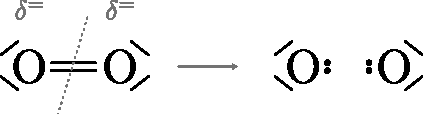
\includegraphics[width=0.7\linewidth, draft=true]{no_O-O2.pdf}
			}{
				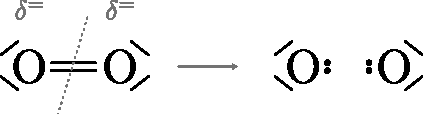
\includegraphics[width=0.7\linewidth]{no_O-O2.pdf}
			}
		\end{center}
		\psw{
			Après répartition fictive des électrons, chaque oxygène est neutre~: $\no{O}
				= 0$
		}
	\end{itemize}
	\vspace{-30pt}
	\tcblower
	\begin{itemize}
		\bitem{Oxygène et hydrogène dans l'eau}~:
		\begin{center}
			\sswitch{
				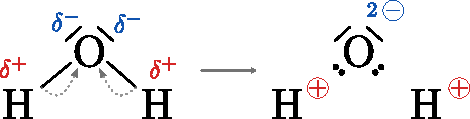
\includegraphics[width=0.7\linewidth, draft=true]{no_O-H2O.pdf}
			}{
				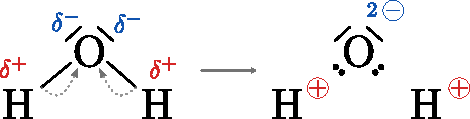
\includegraphics[width=0.7\linewidth]{no_O-H2O.pdf}
			}
		\end{center}
		\psw{
			Après la répartition fictive des électrons,
			% $q_{\ce{O}} = -2e$ et $q_{\ce{H}} = +e$
			$\no{O} = -\myRoman{2} \qqet \no{H} = +\myRoman{1}$
		}
	\end{itemize}
	\vspace{-30pt}
\end{tcb*}

\begin{tcb*}(prop){Nombre d'oxydation}
	\begin{itemize}
		\item Le nombre d'oxydation d'un élément est lié à \textbf{sa structure
			      électronique}~: dans un édifice chaque élément cherche à se
		      rapprocher de la structure des gaz nobles en remplissant ou vidant
		      sa couche de valence, et son nombre d'oxydation est donc
		      \textbf{borné}.
		\item Lors d'une \textbf{oxydation}, \textbf{\no $\nearrow$}~; lors d'une
		      \xul{réduction}, \xul{\no $\searrow$}.
	\end{itemize}
\end{tcb*}

\begin{tcb*}[sidebyside, righthand ratio=.45](exem)<lftt>{Nombre d'oxydation et structure électronique}
	\begin{itemize}
		\bitem{Oxygène}~: \psw{$\chi_{\ce{O}} \nearrow \quad \Ra \quad$ souvent
			chargé $-2e$}
		\bitem{Alcalins}~: \psw{facilement +\myRoman{1}}
		\bitem{Alcalinos-terreux}~: \psw{facilement +\myRoman{2}}
		\bitem{Halogènes}~: \psw{facilement -\myRoman{1}}
		\bitem{Gaz nobles}~: \psw{pas d'oxydation ou de réduction}
	\end{itemize}
	\tcblower
	\begin{center}
		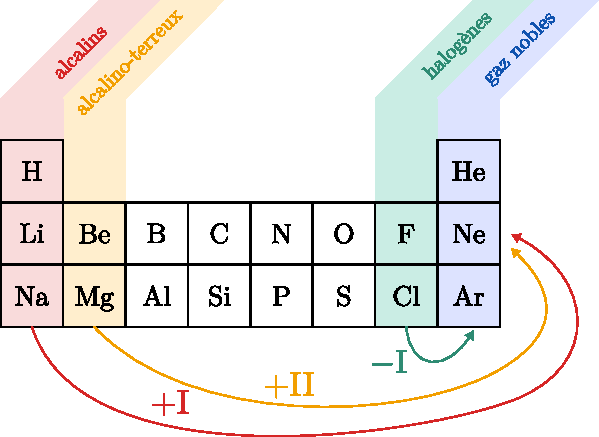
\includegraphics[width=\linewidth]{no_tab.pdf}
	\end{center}
\end{tcb*}

\begin{tcb*}(ror){Règles de calcul nombre d'oxydation}
	\begin{enumerate}
		\item Le \no d'un élément seul est égal à sa charge~;
		\item La somme des \no des élements d'une molécule est égale à la charge
		      de la molécule~;
		      % \item Les éléments d'ions et de molécules homonucléaires ont le même nombre
		      %   d'oxydation de l'élément (???)
		\item En général, dans les molécules et ions complexes, $\no{H} =
			      +\myRoman{1}$~;
		\item En général, dans les molécules et ions complexes, $\no{O} =
			      -\myRoman{2}$ (sauf si cela met en défaut les règles précédentes).
	\end{enumerate}
\end{tcb*}

\begin{tcb*}[sidebyside, lefthand ratio=.26](appl)<lftt>{Calculs de nombres d'oxydation}
	\small
	\begin{itemize}
		\item \ce{Cu}~: \psw{$\no{Cu} = 0$}
		\item \ce{Cu^2+}~: \psw{$\no{Cu} = +\myRoman{2}$}
		\item \ce{Fe^3+}~: \psw{$\no{Fe} = +\myRoman{3}$}
	\end{itemize}
	\tcblower
	\small
	\begin{itemize}
		\item \ce{H2O2}~: \psw{$\no{H} = +\myRoman{1} \Ra 2 \cdot 1 + 2 \cdot
				      \no{O} = 0 \Lra \no{O} = - \myRoman{1}$}
		\item \ce{IO3^-}~: \psw{$\no{O} = -\myRoman{2} \Ra \no{I}+3 \cdot (-2) =
				      -1 \Lra \no{I} = +\myRoman{5}$}
		\item \ce{S2O3^2-}~: \psw{$\no{O} = -\myRoman{2} \Ra 2 \cdot \no{S}+ 3
				      \cdot (-2) = -2 \Ra \no{S} = +\myRoman{2}$}
	\end{itemize}
\end{tcb*}

\begin{tcb}*(expe)<itc>"trans"{Transition}
	Ainsi, l'équilibre entre les espèces d'un couple repose sur la capacité du
	milieu à recevoir ou perdre des électrons~: les couples oxydant-réducteur ont
	donc des caractéristiques électriques.
\end{tcb}

\section{Distribution des espèces d'un couple}
\subsection{Potentiel d'un couple}

\begin{tcb*}[breakable](prop){Formule de \textsc{Nernst}}
	Pour une demi-équation d'oxydoréduction
	\psw{
	\[
		\ce{\alpha Red + \beta H_2O_{\rm(l)} = \gamma Ox + \delta {H}^+_{\rm(aq)} +}
		ne^-
	\]
	}
	le potentiel électrique d'une solution à l'équilibre est donné par la formule
	de \textsc{Nernst}~:
	\psw{
		\[
			E(\ce{Ox}/\ce{Red}) = E^\circ(\ce{Ox}/\ce{Red}) +
			\frac{RT}{n\Fc} \ln
			\frac{a_{\ce{Ox}}^{\gamma}[\ce{H+}]^{\delta}}
			{a_{\ce{Red}}^{\alpha}{c^\circ}^{\delta}}
		\]
	}
	\vspace{-20pt}
	\begin{itemize}
		\item $E$ est le potentiel, et s'exprime en \xul{\psw{volts}}~;
		\item $E^\circ$ est le potentiel standard du couple à la température $T$~;
		\item $n$ le nombre d'électrons échangés (variation du degré d'oxydation)~;
		\item $R$ la constante des gaz parfaits en \xul{\psw{\si{J.K^{-1}.mol^{-1}}}}~;
		\item $T$ la température en \xul{\psw{kelvins}}~;
		\item $\Fc$ la constante de \textsc{Faraday}, représentant la charge
		      électrique d'une mole de protons~:
		      \psw{
			      \[
				      \Fc = e \Nc_A = \SI{96485}{C.mol^{-1}}
				      \quad \Ra \quad
				      \boxed{\frac{RT}{\Fc}\ln 10 \approx \SI{0.059}{V}}
			      \]
		      }
		      \vspace{-30pt}
	\end{itemize}
	D'où la forme commune~:
	\psw{
		\[
			\boxed{
				E(\ce{Ox}/\ce{Red}) = E^\circ(\ce{Ox}/\ce{Red}) +
				\frac{\num{0.06}}{n} \log
				\frac{a_{\ce{Ox}}^{\gamma}[\ce{H+}]^{\delta}}
				{a_{\ce{Red}}^{\alpha}{c^\circ}^{\delta}}
			}
		\]
	}
	\vspace{-15pt}
\end{tcb*}

\begin{tcb*}(rema)<lftt>{Autour de la formule de \textsc{Nernst}}
	\begin{itemize}
		\item Faites attention au passage du logarithme en base $e$ ($\ln$) au
		      logarithme décimal~:
		      \[
			      \log x = \frac{\ln x}{\ln 10}
		      \]
		\item Le potentiel seul n'a pas de sens de manière absolue~: il est défini
		      à une constante près. Il faut donc choisir une référence arbitraire afin
		      de fixer toutes les valeurs. On choisit pour cela le premier couple de
		      l'eau
		      \[
			      E^\circ(\ce{{H}^+_{\rm(aq)}}/\ce{{H_2}_{\rm(g)}}) = \SI{0}{V}
		      \]
	\end{itemize}
\end{tcb*}

\begin{tcb*}[breakable](appl)<lftt>{Calcul de potentiels}
	Donner les potentiels des couples suivants~:
	\begin{itemize}
		\item
		      \leftcenters{%
		      $\ce{{Fe}^2+_{\rm(aq)}}/\ce{Fe_{\rm(s)}}$~:
		      }{%
		      \psw{$\ce{Fe_{\rm(s)} = {Fe}^2+_{\rm(aq)} + 2e^-}$}
		      }
		      % \vspace{-15pt}

		      \psw{
			      \[
				      E = E^\circ \left( \ce{Fe^2+}/\ce{Fe} \right) +
				      \frac{\num{0.06}}{2} \log [\ce{Fe^2+}]
			      \]
		      }
		      \vspace{-15pt}
		\item
		      \leftcenters{%
		      $\ce{{Fe}^3+_{\rm(aq)}}/\ce{{Fe}^2+_{\rm(aq)}}$
		      }{%
		      \psw{$\ce{{Fe}^2+_{\rm(aq)} = {Fe}^3+_{\rm(aq)} + e^-}$}
		      }
		      \vspace{-15pt}
		      \psw{
			      \[
				      E = E^\circ \left( \ce{Fe^3+}/\ce{Fe^2+} \right) +
				      \num{0.06} \log (\frac{[\ce{Fe^3+}]}{[\ce{Fe^2+}]})
			      \]
		      }
		      \vspace{-15pt}
		\item
		      \leftcenters{%
		      $\ce{{MnO_4}^-_{\rm(aq)}/\ce{{Mn}^2+_{\rm(aq)}}}$
		      }{%
		      \psw{
		      $\ce{
			      {Mn}^2+_{\rm(aq)} + 4 H_2O_{\rm(l)}
				      =
				      {MnO_4}^-_{\rm(aq)} + 8 {H}^+_{\rm(aq)} + 5e^-
			      }$
		      }
		      }
		      \vspace{-15pt}
		      \psw{
			      \[
				      E = E^\circ \left( \ce{{MnO_4}^-/\ce{{Mn}^2+}} \right) +
				      \frac{\num{0.06}}{5} \log ( \frac{[\ce{MnO_4^-}][\ce{H+}]^8}{[\ce{Mn^2+}]})
			      \]
		      }
		      \vspace{-15pt}
		\item
		      \leftcenters{%
		      $\ce{{H}^+_{\rm(s)}/\ce{H_2_{\rm(g)}}}$
		      }{%
		      \psw{$\ce{H_2_{\rm(g)} = 2 {H}^+_{\rm(aq)} + 2e^-}$}
		      }
		      \vspace{-15pt}
		      \psw{
			      \[
				      E = E^\circ \left( \ce{H+}/\ce{H_2} \right) +
				      \frac{\num{0.06}}{2} \log ( \frac{[H^+]^2p^\circ}{p_{\ce{H_2}}})
			      \]
		      }
		      \vspace{-15pt}
	\end{itemize}
\end{tcb*}

\subsection{Diagramme de prédominance}
\begin{tcb*}(ror){Diagramme de prédominance}
	\vspace{-10pt}
	\begin{gather*}
		\beforetext{Pour}
		\psw{
			\ce{\alpha Red = \gamma Ox} + n\ce{e^-}
		}
		\qqMath{on a}
		\psw{
			E = E^\circ(\ce{Ox}/\ce{Red}) + \frac{\num{0.06}}{n} \log
			(\frac{a_{\ce{Ox}}^{\gamma}}{a_{\ce{Red}}^{\alpha}})
		}
	\end{gather*}
	On utilisera alors une \textbf{convention de tracé} donnant la valeur de
	$\DS (a_{\ce{Ox}}^{\gamma})/(a_{\ce{Red}}^{\alpha})$ à la limite pour
	trouver $E\ind{lim}$, afin de tracer le diagramme de prédominance~:
	\vspace{-15pt}
	\begin{center}
		\sswitch{
			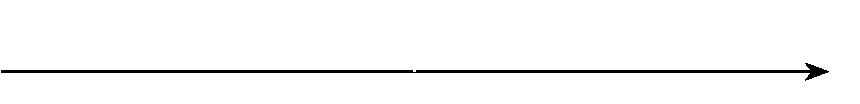
\includegraphics[width=\linewidth]{predom_plain}
		}{
			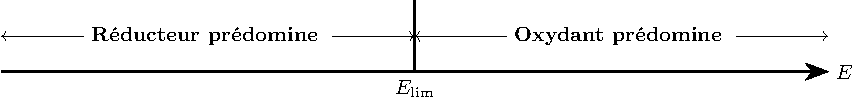
\includegraphics[width=\linewidth]{predom}
		}
		\vspace{-15pt}
		\captionof{figure}{Diagramme de prédominance générique}
	\end{center}
	% \begin{itemize}
	% 	\item à haut potentiel, \xul{\psw{l'oxydant}} domine~;
	% 	\item à bas potentiel, \xul{\psw{le réducteur}} domine.
	% \end{itemize}
\end{tcb*}
\begin{tcb*}(impo){Utilisation des diagrammes redox}
	Ce raisonnement n'est valable \textbf{que pour un couple simple}, sans autres
	espèces dans la demi-réaction. À partir du moment où les protons \ce{H^+}
	interviennent, les diagrammes seront à 2 dimensions~: ce sont les
	\textbf{diagrammes potentiel-pH} (cf.\ chapitre suivant).
\end{tcb*}

\begin{tcb*}[breakable, sidebyside, righthand ratio=.25](defi){Force des oxydants et des réducteurs}
	Comme dans le cas des couples acide-base, on peut parler de la force d'un
	oxydant ou d'un réducteur selon la valeur du potentiel standard~:
	\begin{center}
		\begin{tabular}{ccc}
			\toprule
			$E^\circ$ & \textbf{Oxydant} & \textbf{Réducteur}
			\\
			Élevé     & \psw{fort}       & \psw{faible}
			\\
			Bas       & \psw{faible}     & \psw{fort}
			\\
			\bottomrule
		\end{tabular}
	\end{center}
	\tcblower
	\begin{center}
		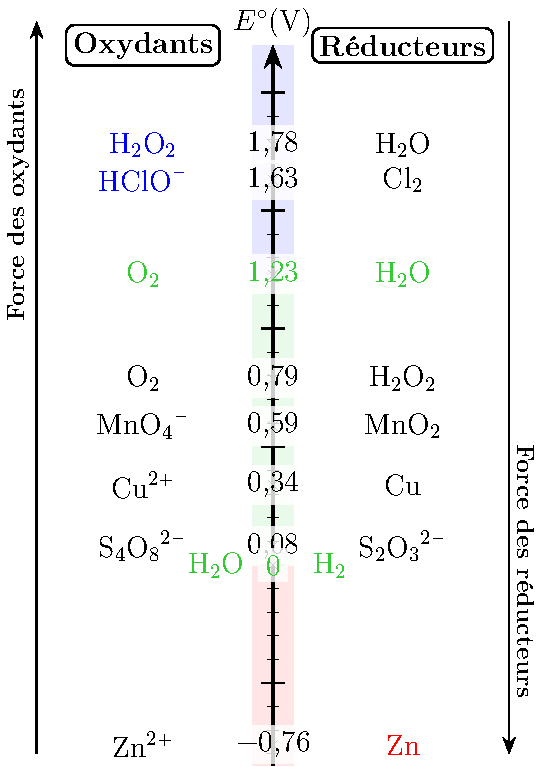
\includegraphics[width=\linewidth]{estand_scale}
		\captionsetup{justification=centering}
		\captionof{figure}{\\Échelle des $E^\circ$}
	\end{center}
\end{tcb*}

\section{Réactions entre couples}
\subsection{Réactions d'oxydoréduction}
\begin{tcb*}[breakable](defi){Réaction d'oxydoréduction}
	Une réaction d'oxydoréduction est une réaction de \textbf{transfert
		d'électrons} entre deux espèces~:
	\psw{
		\[
			\ce{Ox_1 + Red_2 = Red_1 + Ox_2}
		\]
	}
	\vspace{-25pt}
	\begin{itemize}
		\item L'oxydant \xul{\psw{capte}} un (des) électrons, il subit une
		      \xul{\psw{réduction}} et son \no \xul{\psw{diminue}}~;
		\item Le réducteur \xul{\psw{cède}} un (des) électrons, il subit une
		      \xul{\psw{oxydation}} et son \no \xul{\psw{augmente}}.
	\end{itemize}
\end{tcb*}

\begin{tcb*}(impo){Réactions d'oxydoréduction}
	\begin{itemize}
		\item Il n'y a jamais d'électrons dans la réaction bilan~;
		\item La somme des \no est conservée pendant une réaction redox.
	\end{itemize}
\end{tcb*}

\begin{tcb*}(exem)<lftt>{Équilibrage d'équations redox}
	\begin{enumerate}
		\item Écrire et équilibrer la réaction entre $\ce{{Fe}^2+_{\rm(aq)}}$ et
		      $\ce{Cu_{\rm(s)}}$. Les couples mis en jeu sont
		      $\ce{{Cu}^2+_{\rm(aq)}}/\ce{Cu_{\rm(s)}}$ et
		      $\ce{{Fe}^3+_{\rm(aq)}}/\ce{{Fe}^2+_{\rm(aq)}}$.
		\item Écrire et équilibrer la réaction entre $\ce{{Fe}^2+_{\rm(aq)}}$ et
		      $\ce{{MnO_4}^-_{\rm(aq)}}$. Les couples mis en jeu sont
		      $\ce{{MnO_4}^-_{\rm(aq)}}/\ce{{Mn}^2+_{\rm(aq)}}$ et
		      $\ce{{Fe}^3+_{\rm(aq)}}/\ce{{Fe}^2+_{\rm(aq)}}$
	\end{enumerate}
	\tcblower
	\begin{enumerate}
		\item \psw{
			      On écrit les deux demi-équations~:
			      \begin{align*}
				      \ce{Cu_{\rm(s)}}
				       & =
				      \ce{{Cu}^2+_{\rm(aq)} + 2e^-}
				      \tag{1}
				      \\
				      \ce{{Fe}^3+_{\rm(aq)}}
				       & =
				      \ce{{Fe}^2+_{\rm(aq)} + e^-}
				      \tag{2}
				      \\\beforetext{$2 \cdot (2) - (1) \Ra$}
				      \Aboxed{
				      \ce{2 {Fe}^2+_{\rm(aq)} + Cu_{\rm(s)}}
				       & =
				      \ce{{Cu}^2+_{\rm(aq)} + 2 {Fe}^2+_{\rm(aq)}}
				      }
			      \end{align*}
		      }
          \vspace{-15pt}
		\item \psw{
			      On écrit les deux demi-équations~:
			      \begin{align*}
				      \ce{{Mn}^2+_{\rm(aq)} + 4 H_2O_{\rm(l)}}
				       & =
				      \ce{{MnO_4}^-_{\rm(aq)} + 8 {H}^+_{\rm(aq)} + 5e^-}
				      \tag{1}
				      \\
				      \ce{{Fe}^3+_{\rm(aq)}}
				       & =
				      \ce{{Fe}^2+_{\rm(aq)} + e^-}
				      \tag{2}
				      \\\beforetext{$(2) - 5 \cdot (1) \Ra$}
				      \Aboxed{
				      \ce{5{Fe}^2+_{\rm(aq)} + {MnO_4}^-_{\rm(aq)} + 8{H}^+_{\rm(aq)}}
				       & =
				      \ce{5 {Fe}^2+_{\rm(aq)} + {Mn}^2+_{\rm(aq)} + 4 H_2O_{\rm(l)}}
				      }
			      \end{align*}
		      }
          \vspace{-15pt}
	\end{enumerate}
\end{tcb*}

\subsection{Sens de réaction}
Ainsi, comme pour les réactions acide-base, on peut déterminer la stabilité de
certains ions en solution, que ce soit par la superposition des diagrammes de
prédominance ou par la règle du gamma sur une échelle en $E^\circ$~:

\begin{tcb*}[sidebyside, righthand ratio=.25](ror){Sens spontané de réaction}
  Au cours d'une réaction d'oxydoréduction, l'\textbf{oxydant le plus fort} (de
  $E^\circ$ le plus élevé) réagit avec le \textbf{réducteur le plus fort} (de
  $E^\circ$ le plus faible). Cette règle schématise avec la \textbf{règle du
  gamma}, voir Figure~\ref{fig:gamma}.
  \smallbreak
  Cela se détermine aussi avec un diagramme de
  prédominance. En effet, deux espèces de \textbf{domaines disjoints} vont
  réagir ensemble pour donner les espèces qui peuvent exister ensemble au même
  potentiel, voir Figure~\ref{fig:disjoint}.
  \begin{center}
    \sswitch{
          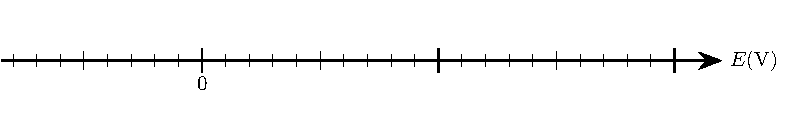
\includegraphics[width=\linewidth]{predom_2-plain}
    }{
    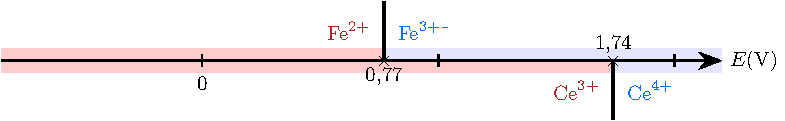
\includegraphics[width=\linewidth]{predom_2}
    }
    \vspace{-15pt}
    \captionof{figure}{Domaines disjoints.}
    \label{fig:disjoint}
  \end{center}
  \tcblower
  \begin{center}
    \sswitch{
          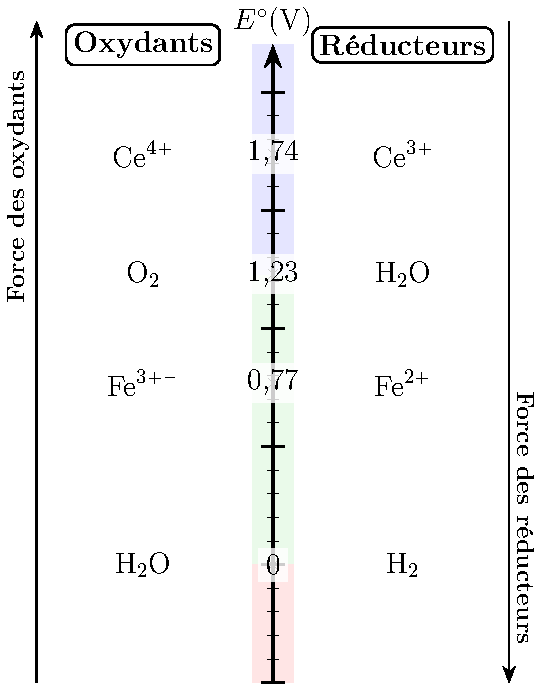
\includegraphics[width=\linewidth]{estand_fece-plain}
    }{
    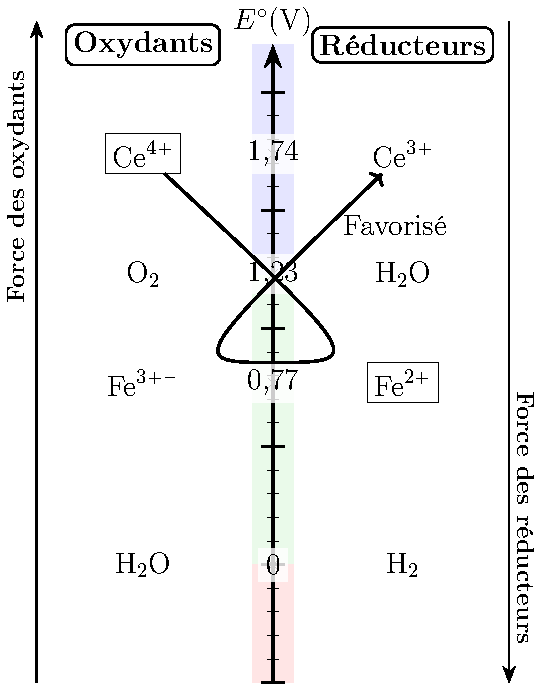
\includegraphics[width=\linewidth]{estand_fece}
    }
    \vspace{-15pt}
    \captionsetup{justification=centering}
    \captionof{figure}{\\Échelle $E^\circ$}
    \label{fig:gamma}
  \end{center}
\end{tcb*}

\subsection{Cas particuliers}
\begin{tcb*}[sidebyside, righthand ratio=.3](defi){Dismutation}
  Une réaction dans laquelle le \textbf{réactif} est \textbf{à la fois oxydant
  et réducteur} est appelée \textbf{dismutation}. On la schématise par la règle
  du gamma ci-contre, et on écrit cette réaction
  \psw{
      \[
      \ce{2A = B+C}
    \]
  }
  \tcblower
  \begin{center}
    \sswitch{
          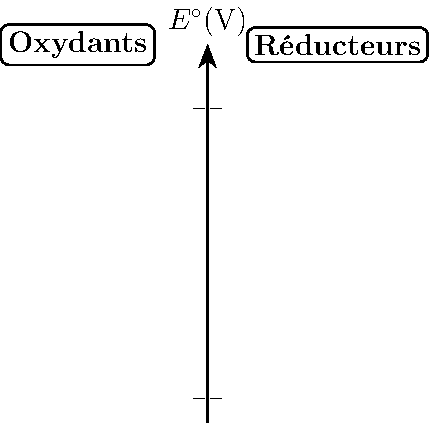
\includegraphics[width=\linewidth]{estand_dismut-plain}
    }{
    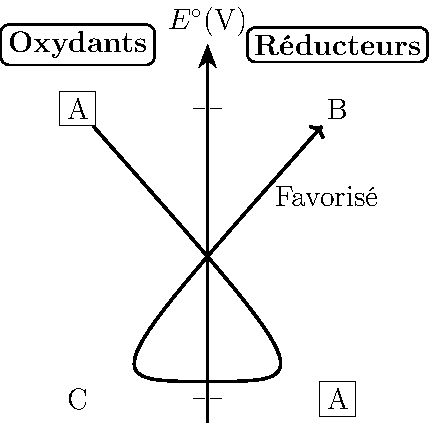
\includegraphics[width=\linewidth]{estand_dismut}
    }
  \end{center}
\end{tcb*}

\begin{tcb*}(exem)<lftt>{Dismutation du fer}
    C'est le cas de l'ion \ce{Fe^2+} qui intervient dans les couples
    \ce{Fe^3+}/\ce{Fe^2+} et \ce{Fe^2+}/\ce{Fe}~: les potentiels standard
    donnent
    \psw{
      \[
        \ce{2 {Fe}^2+_{\rm(aq)} + Fe_{\rm(s)} = 3 {Fe}^2+_{\rm(aq)}}
      \]
    }
\end{tcb*}

\begin{tcb*}[sidebyside, righthand ratio=.3](defi){Médiamutation}
  Une réaction dans laquelle le \textbf{produit} est \textbf{à la fois oxydant
  et réducteur} est appelée \textbf{médiamutation}. On la schématise par la
  règle du gamma ci-contre, et on écrit cette réaction
  \psw{
      \[
      \ce{A + B = 2C}
    \]
  }
  \tcblower
  \begin{center}
    \sswitch{
          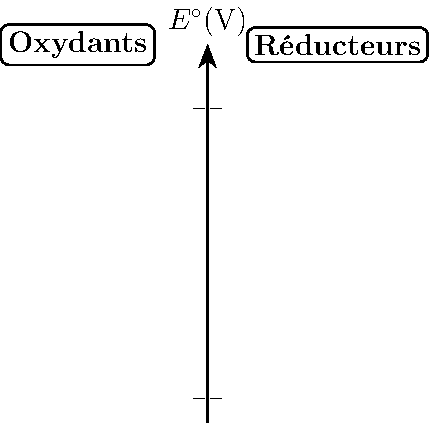
\includegraphics[width=\linewidth]{estand_mediamut-plain}
    }{
    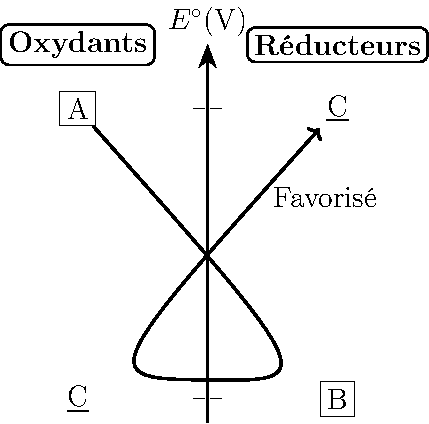
\includegraphics[width=\linewidth]{estand_mediamut}
    }
  \end{center}
\end{tcb*}

\begin{tcb*}(appl)<lftt>{Stabilité par dismutation ou médiamutation}
  Montrer que l'eau oxygénée \ce{H2O2} est instable et que l'eau est stable. On
  donne $E^\circ(\ce{H_2O_2}/\ce{H_2O}) = \SI{1.78}{V}$,
  $E^\circ(\ce{O_2}/\ce{H_2O_2}) = \SI{0.68}{V}$, $E^\circ(\ce{O_2}/\ce{H_2O}) =
  \SI{1.23}{V}$ et $E^\circ(\ce{H_2O}/\ce{H_2}) = \SI{0.0}{V}$.
  \tcblower
  \begin{isd}
    \begin{center}
      \sswitch{
              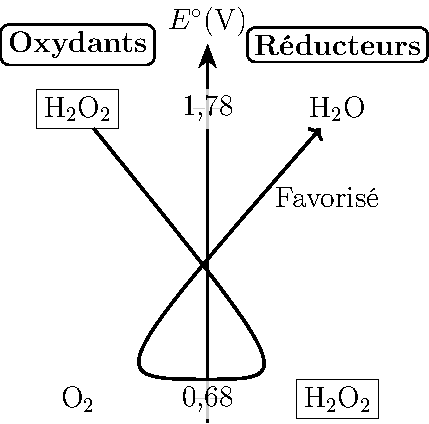
\includegraphics[width=.6\linewidth, draft=true]{estand_dismut-h2o2}
      }{
      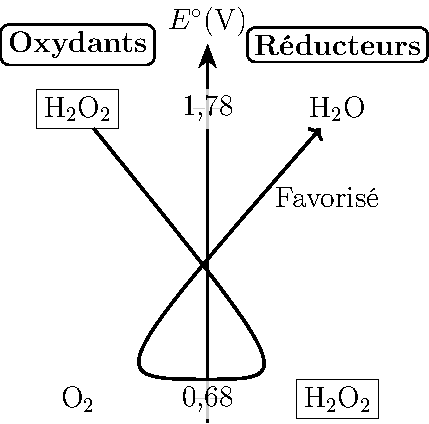
\includegraphics[width=.6\linewidth]{estand_dismut-h2o2}
      }
    \end{center}
    \psw{
          Spontanément, \ce{H2O2} réagit avec lui-même pour former \ce{H2O} et
        \ce{O2}.
    }
    \tcblower
    \begin{center}
      \sswitch{
              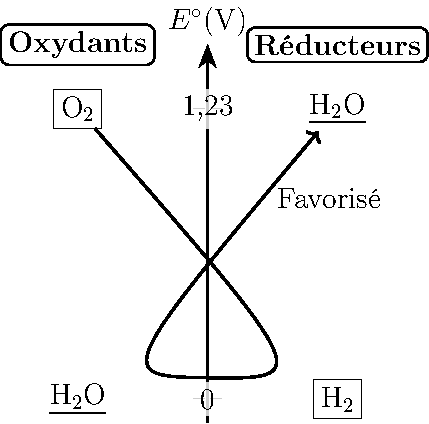
\includegraphics[width=.6\linewidth, draft=true]{estand_mediamut-h2o}
      }{
      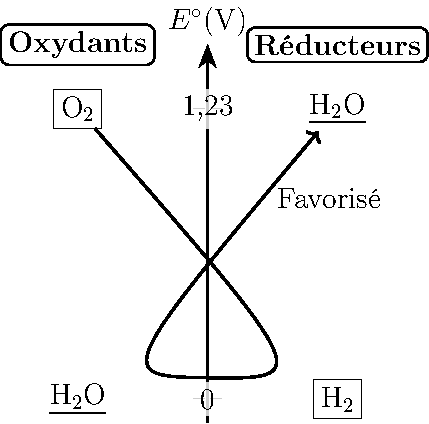
\includegraphics[width=.6\linewidth]{estand_mediamut-h2o}
      }
    \end{center}
    \psw{
          Spontanément, \ce{H2} réagit avec \ce{O2} lui-même pour former \ce{H2O}.
    }
  \end{isd}
\end{tcb*}

\subsection{Calcul de constantes d'équilibre}
\begin{tcb*}(prop){Potentiel en solution}
 Il y a unicité du potentiel en solution~: en présence de plusieurs couples
 rédox dans la solution, les potentiels rédox des différents couples sont égaux
 à l'équilibre. On trouve ainsi la constante d'équilibre d'une réaction~:
 \psw{
   \[
     \ce{Ox_1 + Red_2 = Red_1 + Ox_2}
     \Ra 
     K = \frac{a_{\ce{Red_1}} a_{\ce{Ox_2}}}{a_{\ce{Ox_1}} a_{\ce{Red_2}}}
     \Lra
     \boxed{K = 10^{\frac{n}{\num{0.06}}(E_1^\circ - E_2^\circ)}}
   \]
 }
\end{tcb*}

\begin{tcb*}(impo){Calcul de constantes}
  Ne vous précipitez pas avec les formules, s'il est demandé de
  \textbf{déterminer} il faut faire le calcul~! De même, ne vous trompez pas de
  sens dans la soustraction~: tout dépend du sens de la réaction étudiée.
\end{tcb*}

\begin{tcb*}(appl)<lftt>{Calcul de constante d'équilibre}
    Calculer la constante de réaction entre l'eau oxygénée et l'ion
    permanganate.
    \tcblower
\end{tcb*}

\section{Piles électrochimiques}
Par essence, les réactions d'oxydoréduction sont le siège de l'échange
d'électrons~: en imposant que le transfert se fasse par un circuit électrique
extérieur à la solution, on pourra mettre en évidence et utiliser cette énergie
en réalisant une pile.

\subsection{Présentation}
\begin{tcb*}(defi){Piles électrochimiques}
  On appelle
\end{tcb*}

\begin{center}
  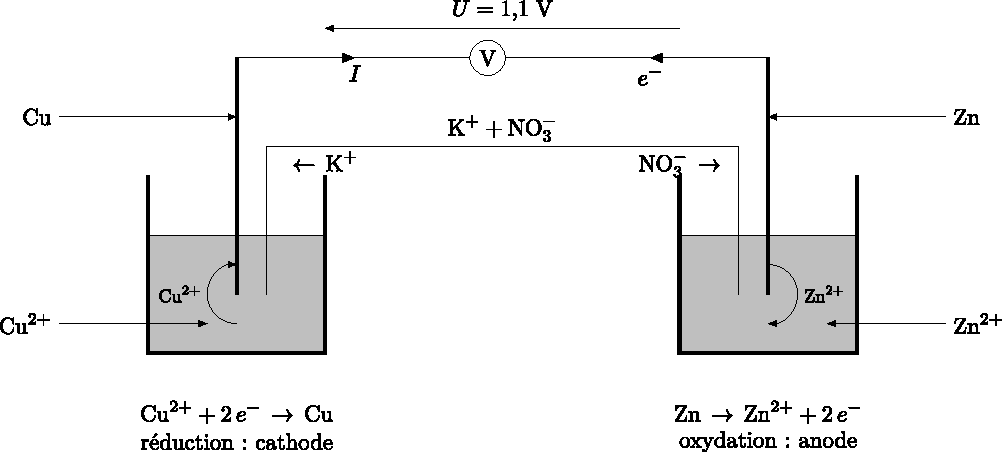
\includegraphics[width=\linewidth]{pile_cu-zn}
\end{center}

\subsection{Potentiel d'électrode}
\begin{tcb*}(defi){Force électromotrice}
  a
\end{tcb*}

\begin{tcb*}(appl)<lftt>{Calcul de la f.e.m.\ de la pile \textsc{Daniell}}
    
\end{tcb*}

\begin{tcb*}(defi){Électrodes de référence}
  
\end{tcb*}

\subsection{Charge totale d'une pile}

\begin{tcb*}(prop){Quantité d'électricité d'une pile}
  \[
    Q = n \xi\ind{eq}\Fc
  \]
\end{tcb*}

\begin{tcb*}(appl)<lftt>{Charge de la pile \textsc{Daniell}}
    
\end{tcb*}


\end{document}
